% paper3_gravity_computation_time.tex
% Gravity as Computation Time on a Spin-1/2 Phase-Bit Lattice
% Author: Thomas Schmiereck
% arXiv category: gr-qc (cross-list quant-ph)

\documentclass[twocolumn,showpacs,preprintnumbers,amsmath,amssymb]{revtex4-2}

\usepackage{amsmath}
\usepackage{amssymb}
\usepackage{graphicx}
\graphicspath{{../figures/}}
\usepackage{booktabs}
\usepackage{hyperref}
\usepackage{physics}
\usepackage{xcolor}
\usepackage{microtype}
\usepackage{nicefrac}

% ── convenience macros ───────────────────────────────────────────────────────
\newcommand{\eps}{\varepsilon}
\newcommand{\cpr}{c'}
\newcommand{\Ot}{2O}
\newcommand{\Ots}{2O^{*}}
\newcommand{\Jint}{J_{\mathrm{int}}}
\newcommand{\bvec}{\mathbf{b}}
\newcommand{\pvec}{\mathbf{p}}
\newcommand{\rvec}{\mathbf{r}}
\newcommand{\vsig}{\boldsymbol{\sigma}}

\begin{document}

\preprint{v3.0.0, November 2026}

\title{Gravity as Computation Time:\\
A Local Budget Rule on a Spin-$\nicefrac12$ Phase-Bit Lattice\\
and its Post-Newtonian Limit}

\author{Thomas Schmiereck}
\email{thomas@schmiereck.de}

\date{November~5, 2026}

% ── Abstract ─────────────────────────────────────────────────────────────────
\begin{abstract}
We ask whether gravity can be modelled as a local limit on how fast each node
of a discrete quantum lattice can compute.
The test particle is a unitary quantum walker on the face-centred-cubic
lattice whose spin is carried by a finite register, the binary octahedral
group $\Ot$: every $60^\circ$ turn rotates the spinor by a quarter turn about
a cube axis.
This gives spin~$\nicefrac12$ with Kramers degeneracy at every momentum, the
belt-trick sign, and exact particle--antiparticle symmetry; a single extra
amplitude, ``reverse the heading without rotating the spin'', is the lattice
Dirac mass $m\beta$ (gap exactly $4\mu$).
Slowing down only the internal clock gives Nordstr\"om gravity; a local wait
buffer per node gives Einstein's 1911 theory (half light bending).
A single node rule---\emph{every process needs each node it involves to be
free}, one node for the clock and two for a hop---produces
$H=N^{2}K+NM$, i.e.\ a spatial metric $A=1/N$ and $\gamma_{\mathrm{PPN}}=1$
to $3\times10^{-4}$ down to $N=0.3$.
Combining loads at a node as independent occupations ($N=\prod_i N_i$) gives
$\beta_{\mathrm{PPN}}=1$ even in the strong field.
A direction-independent drag hop supplies $g_{0i}$ with the coefficient that
the relativity principle demands.
In the full \mbox{3\!+\!1D} walker light is deflected $2.07$ times more strongly
than with waiting alone, the classical orbits of the lattice metric give the
general-relativistic perihelion advance, and a lattice ``gravitational atom''
built in a slab of the 3D walker reproduces the fine structure
$\propto 2\gamma+1$ (de~Sitter) and the Lense--Thirring hyperfine shifts of the
Dirac equation in the corresponding metric to $1$--$4\%$.
We state clearly what is imposed: the field equations for the lapse and the
shift, a vacuum counterterm, and the gyroscope rule.
\end{abstract}

\maketitle

% ─────────────────────────────────────────────────────────────────────────────
\section{Introduction}
\label{sec:intro}
% ─────────────────────────────────────────────────────────────────────────────

In two earlier papers~\cite{schmiereck2026,schmiereck2026b} we showed that a
path-integral lattice with the single rule ``a change of direction costs a
factor $i\eps$'' reproduces relativistic dispersion, a geometric speed of
light, mass, time dilation, and a characteristic internal (crystal angular
momentum) structure.
The present paper adds gravity.

\begin{figure*}[t]
  \centering
  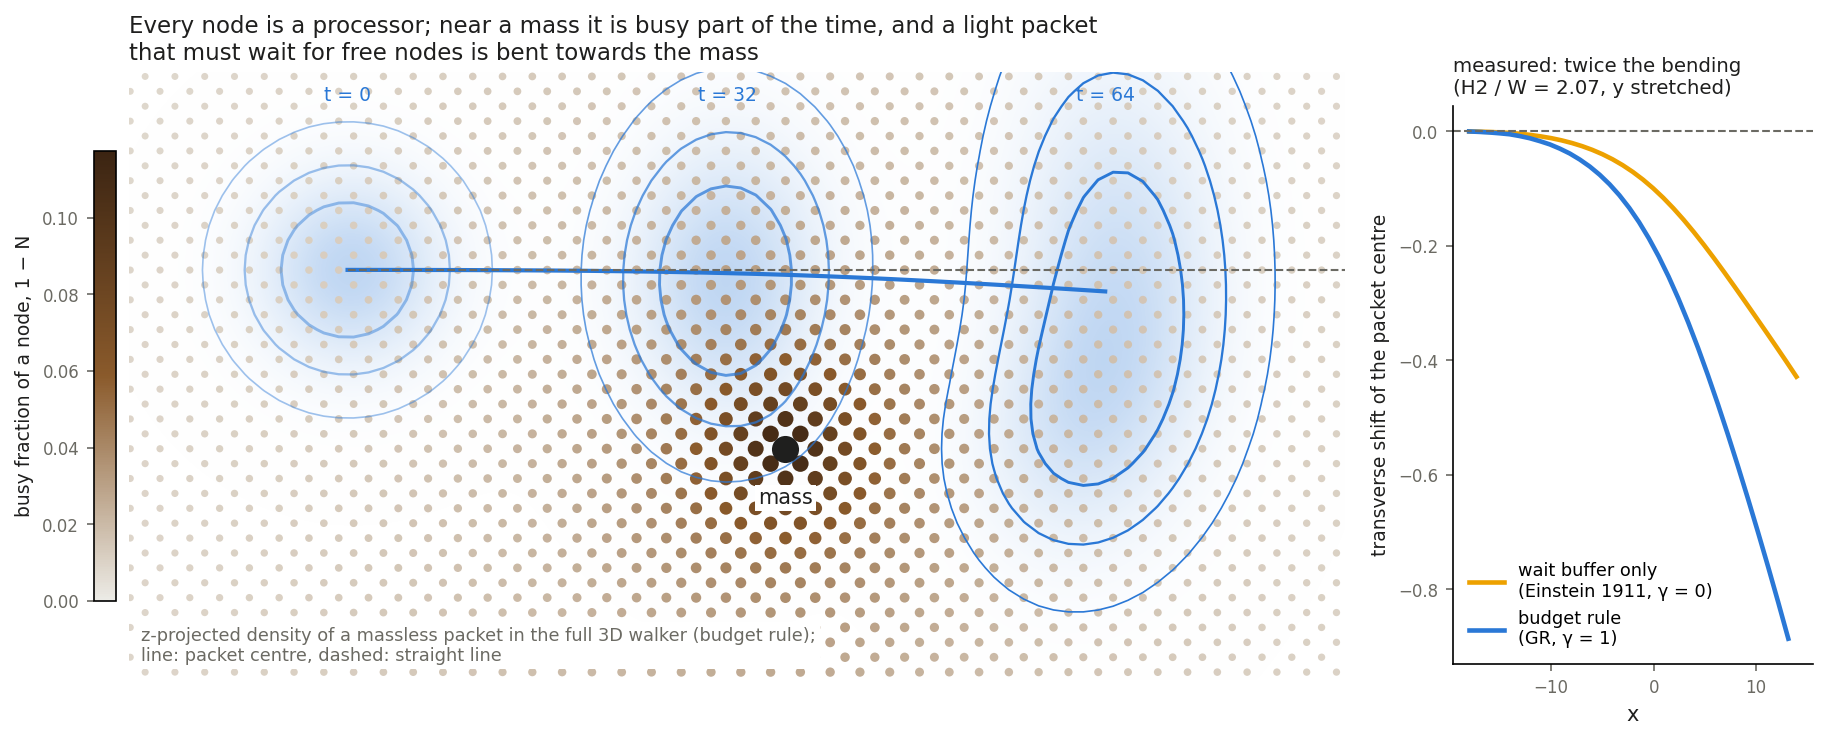
\includegraphics[width=\textwidth]{paper3_lead.png}
  \caption{Light passing a point mass on the phase-bit lattice.
  Left: the $z=0$ plane of the FCC lattice; each node is drawn with its busy
  fraction $1-N$, $N=e^{-U}$, $U=GM/\sqrt{r^{2}+r_c^{2}}$ ($GM=0.25$,
  $r_c=2$).
  Blue: $z$-projected density of a massless packet ($k_0=0.6$, $\sigma=5$,
  impact parameter $12a$) in the full 3D walker with the budget rule
  (Sec.~\ref{sec:gravity}) at three times; the side closer to the mass lags
  behind and the packet centre (solid line) bends towards the mass.
  Right: transverse shift of the packet centre with the wait buffer alone and
  with the budget rule (vertical scale stretched); the deflection ratio is
  $2.07$, the GR value $1+\gamma=2$ (Sec.~\ref{sec:3d}).}
  \label{fig:lead}
\end{figure*}

The guiding idea is simple and old in spirit: if the world is a computation,
a region that has more to compute may compute more slowly
(Fig.~\ref{fig:lead}).
In general relativity (GR) the static weak field is
$ds^{2}=-N^{2}dt^{2}+A^{2}d\mathbf{x}^{2}$ with lapse $N=1-U$ and spatial
metric $A=1+\gamma U$, where $U=GM/rc^{2}$ and $\gamma=1$.
A lapse alone ($\gamma=0$) is Einstein's 1911 theory and bends light by half
the observed amount~\cite{einstein1911}.
The question is therefore not whether ``slower computation'' can mimic a
redshift---it obviously can---but whether a \emph{local} rule on a lattice
also produces the spatial metric, and with it the parameters $\gamma$ and
$\beta$ of the parametrised post-Newtonian (PPN) formalism~\cite{will2014}.

We proceed in three steps.
Section~\ref{sec:particle} builds the test particle: a unitary
\mbox{3\!+\!1D} quantum walker~\cite{aharonov1993,strauch2006} with spin
$\nicefrac12$ from a finite register and a time-reversal-invariant Dirac mass.
Section~\ref{sec:gravity} climbs the ladder from a slowed clock (Nordstr\"om)
via a local wait buffer (Einstein 1911) to the budget rule ($\gamma=\beta=1$)
and adds the gravitomagnetic shift (overview in Fig.~\ref{fig:ladder}).
Sections~\ref{sec:3d} and~\ref{sec:atom} test the result in the full 3D walker:
light deflection, Newton's law, perihelion advance, Lense--Thirring, and the
fine and hyperfine structure of a lattice gravitational atom.
Section~\ref{sec:discussion} separates what follows from the rules from what
was put in by hand and lists the lattice-specific signatures.

All results are reproducible with the scripts and data in the public
repository~\cite{repo}; every number quoted below is taken from a stored run.

% ─────────────────────────────────────────────────────────────────────────────
\section{The particle: spin $\nicefrac12$ from a finite phase-bit register}
\label{sec:particle}
% ─────────────────────────────────────────────────────────────────────────────

\subsection{Phase bits}

On the hexagonal lattice of Ref.~\cite{schmiereck2026} the amplitude of a path
is $\prod(i\eps)$ over its turns, i.e.\ a sum of \emph{integer} path counts
weighted by $i^{T}$, where $T$ is a $\mathbb{Z}_4$ turn counter.
If a turn by $n\cdot60^\circ$ also advances a phase bit $p\in\mathbb{Z}_4$ by
$n$, only $12$ of the $24$ labels $(d,p)$ are reachable: the label space is
$\mathbb{Z}_{12}$, the double cover of the six headings, and every closed walk
of odd winding returns with the sign $-1$ (checked against exact enumeration
up to length~$9$).
In 2D this is the $\alpha=\nicefrac12$ spinor point of the turning-phase model
and gives Kramers doublets, but a mass term necessarily breaks time reversal
(the \mbox{2\!+\!1D} parity anomaly; we verified that $500$ random T-even terms
never split the Dirac pair, splitting $\le2.9\times10^{-15}$).

\subsection{The $\Ot$ register in 3D}

In 3D the holonomy of the minimal SU(2) transport along the cuboctahedron of
FCC directions is not quantised: the transports generate an infinite group.
We replace each minimal rotation between neighbouring headings ($60^\circ$
apart) by the closest element of the octahedral group.
It is unique: the quarter turn about a cube axis,
\begin{equation}
  Q(d\!\to\!d') = \frac{1+i\,\mathbf{n}\cdot\vsig}{\sqrt2},
  \label{eq:Q}
\end{equation}
with fidelity $0.8165$ against $0.5774$ for the competing $120^\circ$ rotation.
The $48$ matrices $Q$ generate the binary octahedral group $\Ot$ (the Clifford
group of one qubit up to phases).
Of the $12\times48$ conceivable labels (heading, group element) only $48$ are
reachable, four per heading---again a $\mathbb{Z}_4$ phase bit, now
transforming non-abelianly when the heading changes.
The integer path-count table, read out with the irreducible representations of
$\Ot$, reproduces the floating-point walk to $1.8\times10^{-15}$ and contains
spin $0$, $\nicefrac12$, $1$ and $\nicefrac32$ sectors in one table.

The coin is $C=\exp(i\eps G)$ with $G=\sum|d'\rangle\langle d|\otimes Q(d\!\to\!d')$.
The spin-$\nicefrac12$ walker is unitary ($9\times10^{-16}$), causal
($\max|v_g|=1.687<c=\sqrt3$), Kramers degenerate at every $k$
($6\times10^{-15}$), and the heading triangle and square carry holonomies
$\pi$ and $2\pi$ (all closed walks up to length~$8$ return with $-1$).
In contrast to the minimal-SU(2) walker the spectrum is exactly symmetric under
$E\leftrightarrow-E$ ($3.6\times10^{-15}$ against $0.22$): the traceless
holonomy of the triangles removes odd cycles from the spectral traces.

\subsection{Mass as reversal without spin rotation}

The lowest level is a fourfold Dirac point,
$H_{\mathrm{eff}}=E_0+\sum_i k_i\Gamma_i$ with
$\{\Gamma_i,\Gamma_j\}=2\cpr^{2}\delta_{ij}$, $\cpr=c/3$.
A local term $V$ opens a gap iff the traceless part of its projection
anticommutes with all $\Gamma_i$.
Scanning all couplings between headings at $60^\circ$, $90^\circ$,
$120^\circ$, $180^\circ$ shows: terms that transport the spin correctly only
shift the Dirac point; masses appear exactly where the spin is \emph{not}
rotated along with the heading.
The simplest is the $180^\circ$ reversal with identity on the spin, which is
the inversion $\Pi$ itself:
\begin{equation}
  C=\exp\!\big(i(\eps G+\mu\,\Pi)\big),\qquad [\Pi,G]=0 .
\end{equation}
It is the lattice version of $m\beta$: the gap is exactly $4\mu$ at every
order, P, T $=\Pi\Theta$ and PT are conserved, and with $\Ot$ the
$E\leftrightarrow-E$ symmetry survives ($4\times10^{-15}$).
\emph{Mass is the amplitude to reverse the direction of motion without turning
the spin.}

The massive quartet carries a common background $-\alpha k^{2}$ in addition to
the Dirac structure.
A coupling between headings at $90^\circ$ with spin transport, $\lambda\eps
W_{90}$, commutes with $G$ and cancels it ($\lambda^{*}=-3.204$ at
$\eps=0.3$); we call the compensated model $\Ots$.
At $\eps=0.3$ its massive band is Dirac to $-0.3\%/-1.0\%$ ($\mu/\eps=0.1$,
$k=0.2/0.4$) and isotropic.
All gravity results below use $\Ots$ at $\eps=0.3$ with $\Delta t=\nicefrac12$;
its limiting speed is $\cpr=c/3$ and $m=2\mu$.

% ─────────────────────────────────────────────────────────────────────────────
\section{Gravity as computation time}
\label{sec:gravity}
% ─────────────────────────────────────────────────────────────────────────────

\begin{figure*}[t]
  \centering
  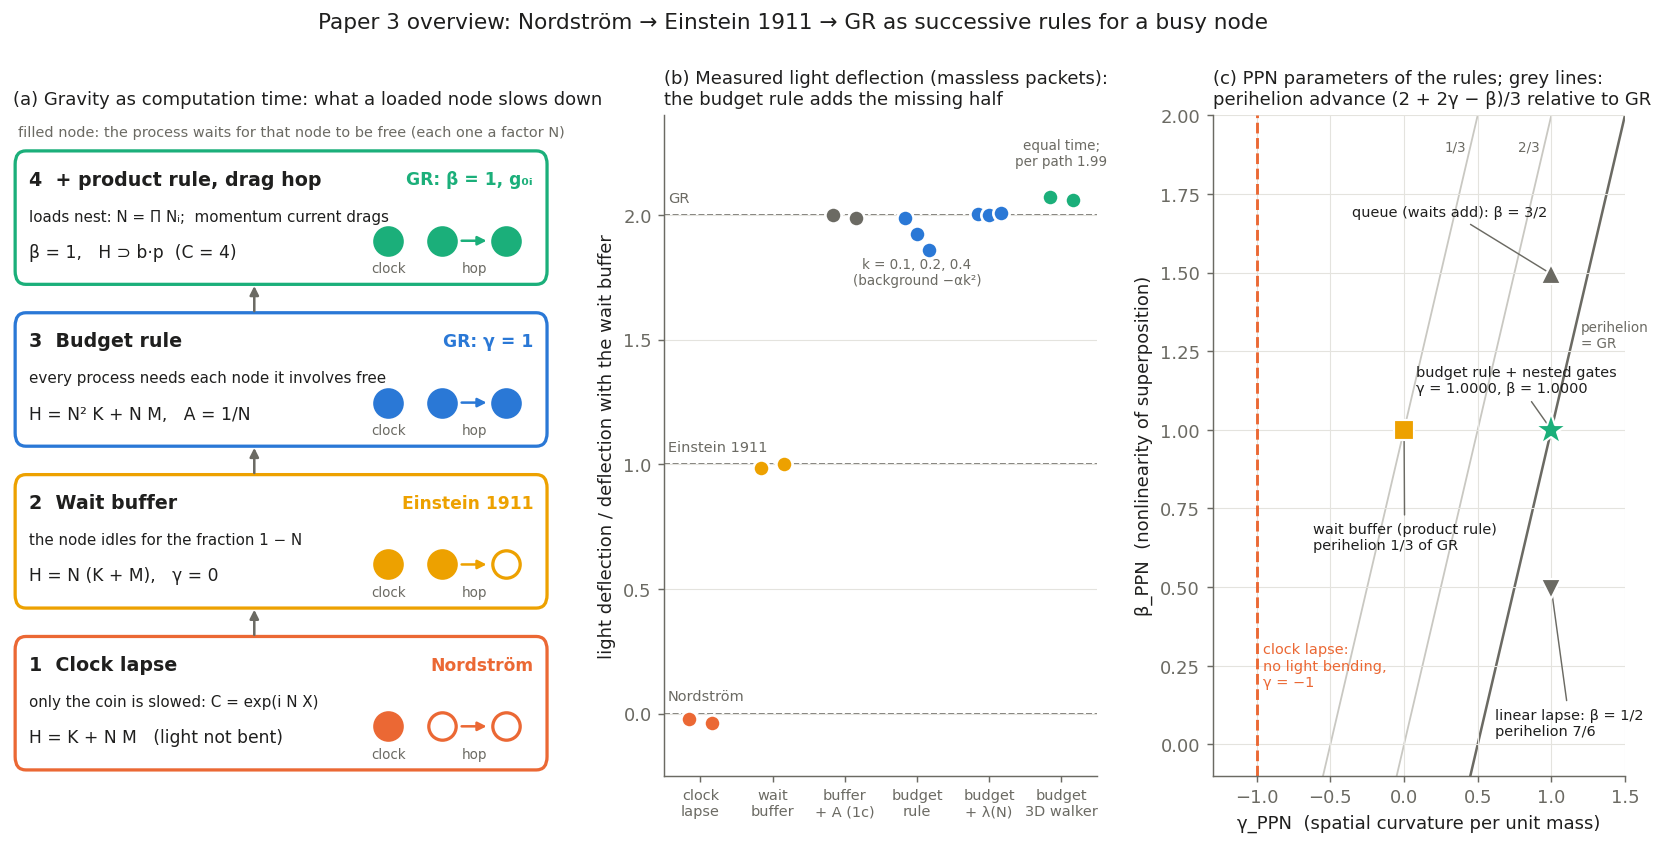
\includegraphics[width=\textwidth]{paper3_ladder.png}
  \caption{Overview of the ladder.
  (a) What a loaded node slows down on each rung; a filled node means the
  process waits for that node to be free, each contributing a factor $N$.
  (b) Measured deflection of massless packets relative to the wait buffer
  (Einstein 1911): clock lapse and global full lapse on the same chain,
  local buffer against the global full lapse, Exp.~1c with $A$ set by hand,
  the budget rule on the chain without and with the $\lambda(N)$
  compensation ($k=0.1,0.2,0.4$), and the full 3D walker (equal time).
  (c) PPN parameters of the rules with lines of constant perihelion advance;
  only the budget rule with nested gates lies on the GR point.}
  \label{fig:ladder}
\end{figure*}

\subsection{The vacuum must not gravitate}

A lapse rescales quasi-energies.
In $\Ots$ the Dirac quartet sits at the Floquet offset $E_c=+1.02$ while the
mass is $0.06$; without correction the particle would fall $18$ times too
strongly.
We therefore add a local vacuum counterterm $-\eps\,l_v\openone$ that puts
the Dirac point at $E=0$.
Then the passive equivalence ratio $R'=E_0/(m^{*}\cpr^{2})$ is $0.997$ for both
particle and antiparticle ($\mu/\eps=0.1$); without the background
compensation they would fall differently ($0.73$ vs $1.20$).
A residual offset $\delta$ gives $R'=1\pm\delta/m$, measured on the lattice to
three digits---the counterterm is forced, not optional.

\subsection{Clock lapse: Nordstr\"om}

Slowing only the coin, $C(\rvec)=\exp(iN(\rvec)X)$, is exactly local and unitary.
On a chain of $160$ FCC layers with $N=1+gx$ resting massive packets fall,
moving ones less ($\kappa=(m/E)^{2}=1/\gamma^{2}$), and massless packets not
at all ($a_x=+0.1\times10^{-4}$ vs $-5.9\times10^{-4}$ at rest).
This is Nordstr\"om's scalar theory: no light bending.

\subsection{A local wait buffer: Einstein 1911}

To slow \emph{everything} locally, each state $(x,d,s)$ receives a buffer
partner at the same node:
\begin{equation}
  U = R(a)\,\big[\,S C \oplus (-1)\,\big],\qquad
  R(a)=\cos a+i\sin a\,\sigma_x .
  \label{eq:buffer}
\end{equation}
The active register makes a normal step, the buffer waits with phase $-1$, and
$R(a)$ mixes the two on the node.
Because $R(a)$ is the identity on the internal index, every walker eigenphase
$\theta$ maps exactly to
\begin{equation}
  f_a(\theta)=\tfrac{\theta}{2}+\arcsin\!\big(\cos a\,\sin\tfrac{\theta}{2}\big)
  \approx N\theta,\qquad N=\tfrac{1+\cos a}{2},
\end{equation}
(checked to $4\times10^{-15}$).
Near $E=0$ the whole quasi-energy---clock \emph{and} propagation---is scaled by
$N$, and the buffer holds exactly the fraction $1-N$ of the amplitude: a node
with lapse $N$ spends the fraction $1-N$ of its time waiting.
Only the buffer phase $\pi$ keeps the vacuum at $E=0$ for every $N$; any other
phase makes the vacuum energy $N$-dependent, and it would gravitate.
On the chain everything now falls alike, light included
($a/(-gN_0^{2}\cpr^{2})=0.86/0.85/0.79$ for massive packets at
$k_y=0/0.3/0.6$, $0.72/0.88$ for massless ones), reproducing the global full
lapse $\tfrac12\{N,H\}$: Einstein 1911.

More generally, for \emph{any} local wait scheme the lapse is the active weight
of the vacuum fixed vector (Hellmann--Feynman; random two-buffer schemes agree
to $10^{-3}$), and any combination of wait buffers---also separate ones for hop
and coin---scales hop and clock alike: $\gamma=0$.
Waiting alone can never produce a spatial metric.

\subsection{The budget rule: $\gamma=1$}
\label{sec:H2}

The clock (coin, mass rotation) involves one node; a hop involves two,
departure and arrival.
We postulate: \emph{a node is free with weight $N$, and every process needs all
nodes it involves to be free.}
Two local gates implement this:
\begin{align}
  W(a) &= R(a)\,[\,V\oplus(-1)\,] && \text{(busy: idle)}\nonumber\\
  H(b) &= R(b)\,[\,SC\oplus(-C)\,] && \text{(hop refused)}\nonumber\\
  U &= W(a)\,\big[\,H(b)\,(SC\oplus -C)\oplus(-1)\,\big] .
\end{align}
With $N_w=N_h=N$ the stay gate slows only the hop, the wait gate slows both,
and the band obeys
\begin{equation}
  H = N^{2}K + N M ,
  \label{eq:H2}
\end{equation}
with $K$ the massless and $M$ the mass part.
This is the weak-field metric with $A=1/N$.
Measured on the band (gap/$m$ and slope/$\cpr$ extrapolated to $k\to0$):

\begin{center}
\begin{tabular}{ccc}
\toprule
$N$ & $A$ & $\gamma=-\ln A/\ln N$\\
\midrule
$0.95$ & $1.0526$ & $0.9997$\\
$0.9$ & $1.1111$ & $0.9998$\\
$0.7$ & $1.4285$ & $0.9999$\\
$0.5$ & $2.0000$ & $1.0000$\\
$0.3$ & $3.3333$ & $1.0000$\\
\bottomrule
\end{tabular}
\end{center}

\noindent
So $g_{00}g_{rr}=-1$ holds into the strong field.
The general count is $\gamma=(n_{\mathrm{hop}}-n_{\mathrm{clock}})/n_{\mathrm{clock}}$;
for one and two nodes it is exactly $1$, and since every hop in every direction
involves two nodes the metric is isotropic.
In Bloch-sphere language each gate is a register qubit whose fixed vector has
polar angle $a$; the lapse is its active weight $\cos^{2}(a/2)$.

\emph{Price and repair.}
The stay gate adds a band curvature
$-\alpha k^{2}$, $\alpha=0.245\,N_h(1-N_h)$, of order $\Delta t$.
Because $\lambda$ changes only this background (Dirac point, gap and velocity
fixed to $2\times10^{-4}$), a node that retunes $\lambda(N)$
($\Delta\lambda\approx3.3(1-N)$) removes it for $N\gtrsim0.4$.
On the chain light is then deflected twice as strongly as with waiting alone,
$(a_{H2}/N_0^{2})/a_{1b}=2.005/1.998/2.007$ at $k=0.1/0.2/0.4$,
i.e.\ $\gamma=1.00\pm0.007$; massive Dirac-regime packets give
$\gamma=0.99$--$1.00$ (Fig.~\ref{fig:H2}).

\begin{figure*}[t]
  \centering
  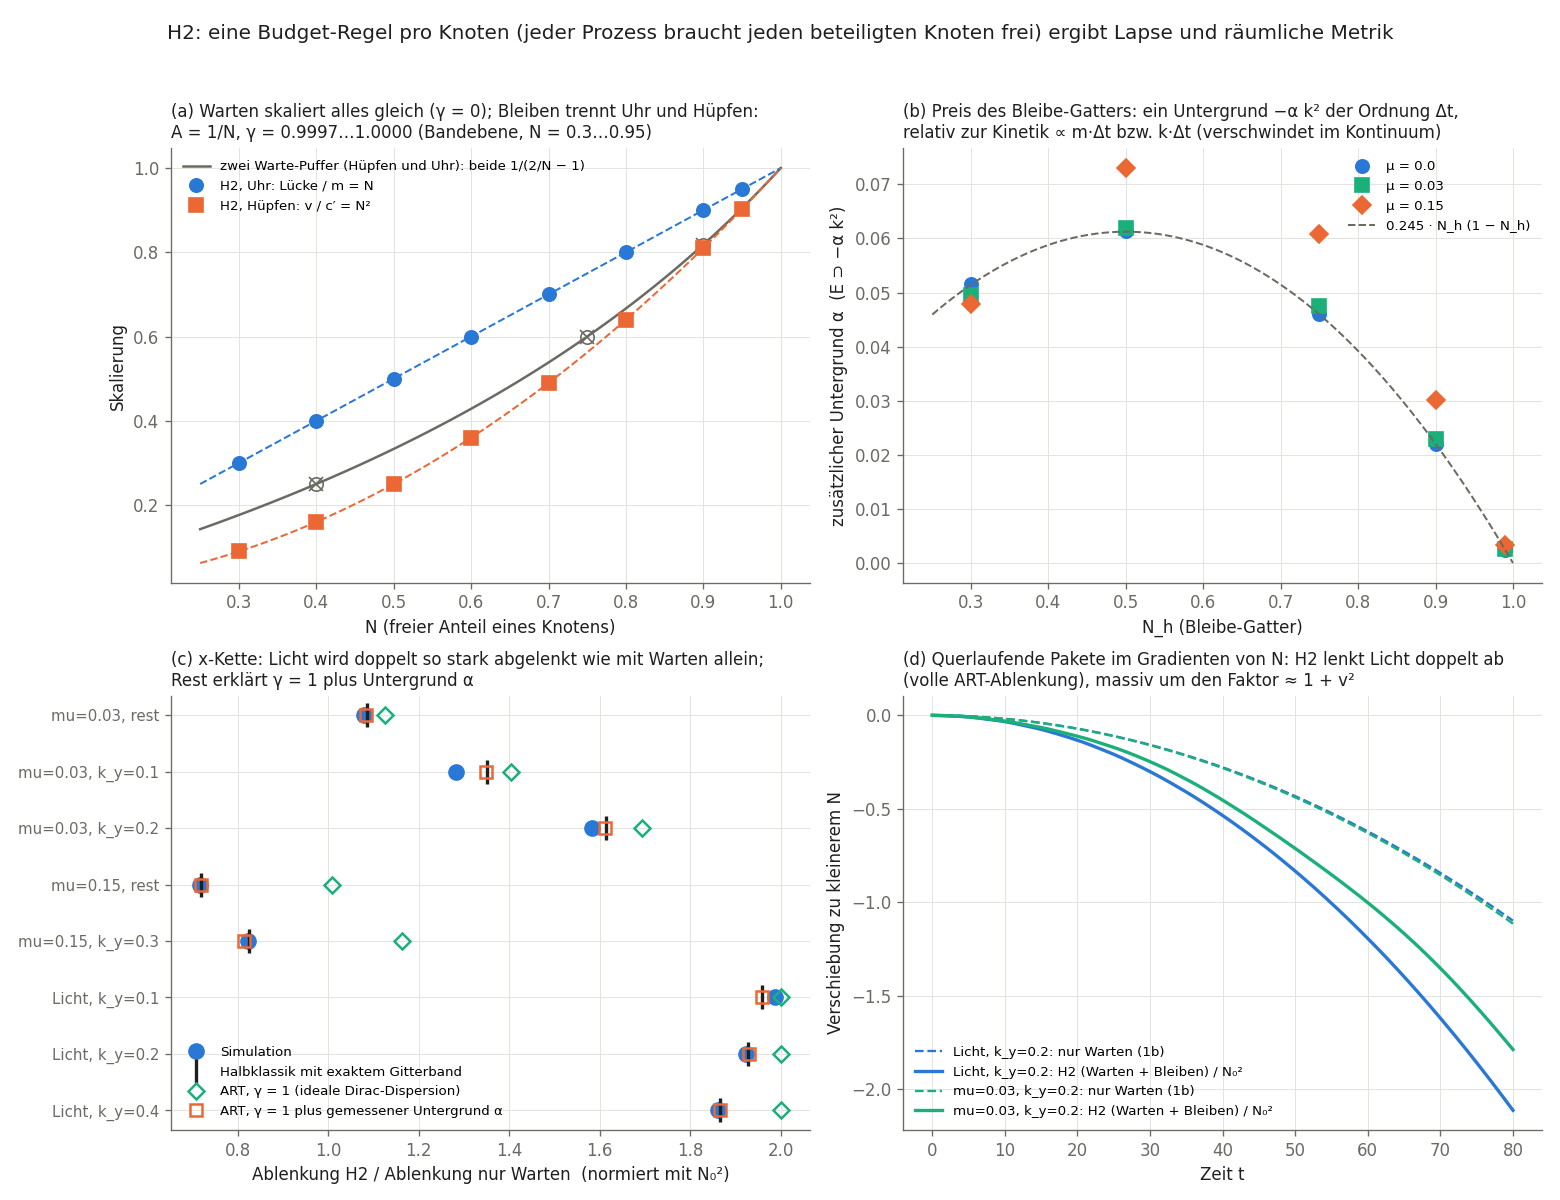
\includegraphics[width=0.92\textwidth]{phase_bit_s4_open8.png}
  \caption{The budget rule (H2).
  Waiting alone is always a pure lapse; the stay gate slows only hops, giving
  $H=N^{2}K+NM$, $A=1/N$ and $\gamma_{\mathrm{PPN}}=1$; on an $x$-chain light is
  deflected twice as strongly as with the wait buffer (Einstein 1911).}
  \label{fig:H2}
\end{figure*}

\subsection{Combining loads: $\beta=1$}

In isotropic PPN gauge $\ln N=-U+(\beta-1)U^{2}$.
If the field law is linear in the sources, $\beta$ is fixed by how two loads
combine at one node:
\begin{equation}
  \beta-1=\frac{\ln N_{12}-\ln N_1-\ln N_2}{2\ln N_1\ln N_2}.
\end{equation}
We measured three composition laws on the band:
\begin{center}
\begin{tabular}{lcc}
\toprule
law & gate & $\beta$\\
\midrule
linear, $N=1-\sum U_i$ & one & $0.20$--$0.50$\\
queue, $N^{-1}-1=\sum(N_i^{-1}-1)$ & parallel & $1.37$--$1.50$\\
\textbf{product}, $N=\prod N_i$ & \textbf{nested} & $\mathbf{1.0000}$\\
\bottomrule
\end{tabular}
\end{center}

\noindent
Nested gates---a state must be free for \emph{each} load---give $\beta=1$ to
$10^{-4}$ up to $N_{12}=0.49$, and keep $A=1/(N_1N_2)$.
This is the same logic as the budget rule itself (a hop needs $N\cdot N$, a
state needs $N_1\cdot N_2$).
The field must therefore couple as $N=N_0e^{\Phi}$, not $N_0(1+\Phi)$.
Queues and linear superposition are excluded by the perihelion of Mercury and
lunar laser ranging~\cite{will2014}.

\subsection{The source: computational load}

The source of $\Phi$ is the local load
$e(x)=\mathrm{Re}\,\psi^{\dagger}i(U\psi-\psi)/\Delta t$ (zero in the vacuum)
and the mass load $e_M=\mu\,\mathrm{Re}[i(U\psi)^{\dagger}\partial_\mu U\psi]/\Delta t$,
both local.
The combination $s=2e-e_M$ equals $T_{00}+T_{ii}$: a moving source pulls with
$1.887/1.964$ against $1+v^{2}=1.892/1.970$, light with $2$.
The mass load is the proper time, $e_M/m=d\tau/dt=N\sqrt{1-v^{2}}$ (lattice band
to $0.9\%$, $40$ cases), and its space-time integral is $m\tau=-S$.
A resting source in a potential loads with $N m$ ($2\times10^{-5}$); together
with the product rule this gives
\begin{equation}
  g_{00}=-1+2U^{*}-2U^{*2}+3\Phi_1^{*}-2\Phi_2^{*}
\end{equation}
in the conserved density $\rho^{*}$, which is the 1PN $g_{00}$ of GR.
For antimatter the load of the lower band is negative; only the hole picture
(load relative to the filled sea) gives normal attraction ($\pm1.858\times10^{-4}$
for a particle--antiparticle pair), at the price of normal ordering the sea.
With a local wave equation $\Phi_{tt}=c_g^{2}(\nabla^{2}\Phi-\kappa s)$,
$c_g=\cpr$, a test particle starts to fall only after the light travel time;
in 3D the static field is $1/r$ to $0$--$2\%$ and does not grow secularly.

\subsection{Gravitomagnetism: the drag hop}
\label{sec:g0i}

With scalars $N$ and $A$ only, the lattice would be a preferred frame for
gravity.
For two sheets with speeds $v_s$, $v_t$ the transverse force carries the factor
$(1+v_s^{2})(1+v_t^{2})-Cv_sv_t$, and co-moving bodies cannot detect their
motion ($a\propto1/\gamma^{3}$) only if $C=4$, the GR value.
A heading-dependent stay gate gives a linear term but splits Kramers pairs and
shifts the vacuum: in this walker the internal index \emph{is} the direction
of motion.
The working solution is a \emph{direction-independent drag hop}: every node
hands a small fraction of every state, whatever its heading, to its neighbour
along the momentum current.
It generates $H\supset\bvec\cdot\pvec$ exactly ($5\times10^{-15}$ on the band),
leaves the Dirac point and Kramers pairs untouched, and with
$\bvec\propto4\cpr^{2}\kappa\,\nabla^{-2}(\text{momentum density})$ gives on a
$640$-layer chain: parallel light beams $0.019$ (packet GR $0.022$; without
$g_{0i}$ $0.053$), antiparallel $1.99$, co-moving sheets
$a(k,k)/a(0,0)=0.669/0.319$ against $0.675/0.339$ (without $g_{0i}$:
$1.77/3.63$).
Causally propagated ($\Phi$ and $\bvec$ as wave equations), parallel light
beams feel nothing at any time; an instantaneous $\bvec$ next to a retarded
$\Phi$ would give a superluminal repulsion.

In 3D the drag is a brick wall of real bond rotations between FCC neighbours,
angle $\Delta t\,(\bvec\cdot\mathbf{s})/(8\ell^{2})$ at the bond midpoint,
exactly unitary and strictly local.
A rotating ball gives the GR dipole $\bvec=2\cpr^{2}(\kappa/4\pi)\,\mathbf{J}\times\rvec/r^{3}$
($0.99$ at $r=8$).
In a rigidly rotating drag field a packet is carried along ($0.00406$ against
$\Omega=0.004$), but its spin is not ($0.00026$): $\bvec\cdot\pvec=\Omega L_z$
couples to the orbit only.
A gyroscope needs the additional rule
$\exp(-i\Delta t\,\tfrac12\nabla\times\bvec\cdot\Jint)$ with the lattice's own
rotation generator $\Jint=(2i/\pi)\log R_{90}$ ($R_{90}$: heading permutation
times spin rotation, commutes with the coin).
It has $g=1$ on every spin-$\nicefrac12$ doublet, and the spin then turns with
$0.00399$.
The bare spin index $P(\openone\otimes\vsig/2)P$ would give $g=-\nicefrac13$
for the particle: most of its spin sits in the headings.

% ─────────────────────────────────────────────────────────────────────────────
\section{Tests in the full 3+1D walker}
\label{sec:3d}
% ─────────────────────────────────────────────────────────────────────────────

\subsection{Light deflection by a point mass}

The full 3D walker runs on a periodic $112\times88\times80$ box ($7.9\times10^{5}$
nodes, four registers, complex64), with $U=GM/\sqrt{r^{2}+r_c^{2}}$,
$GM=0.25$, $r_c=2$, $N=e^{-U}$, and coins tabulated in $48$ classes of $N$.
A massless packet ($k_0=0.6$, $\sigma=5$) passes the mass at impact parameter
$b$.
Both Kramers partners give the same deflection to $10^{-5}$.

\begin{center}
\begin{tabular}{lcccc}
\toprule
$b$ & rule & $\Delta k_y$ sim. & sim./local force & H2/W\\
\midrule
$7.35$ & W & $-0.02174$ & $1.018$ & \\
$7.35$ & H2 & $-0.04503$ & $1.027$ & $\mathbf{2.071}$\\
$12.25$ & W & $-0.01907$ & $1.000$ & \\
$12.25$ & H2 & $-0.03925$ & $1.012$ & $\mathbf{2.058}$\\
\bottomrule
\end{tabular}
\end{center}

\noindent
The budget rule doubles the deflection in 3D: $4GM/b$ against Einstein's
$2GM/b$.
The excess over $2$ is a time effect (light is slower in H2, $\cpr N^{2}$, and
spends longer near the mass); per distance travelled the straight-ray estimate
is $1.99/1.98$.
The local force $n_sN^{n_s}\cpr\langle|k|\rangle\partial_yU$ ($n_s=1$ for W,
$2$ for H2), averaged over the simulated density, matches to $\le2.7\%$
(Fig.~\ref{fig:3d}).

\begin{figure*}[t]
  \centering
  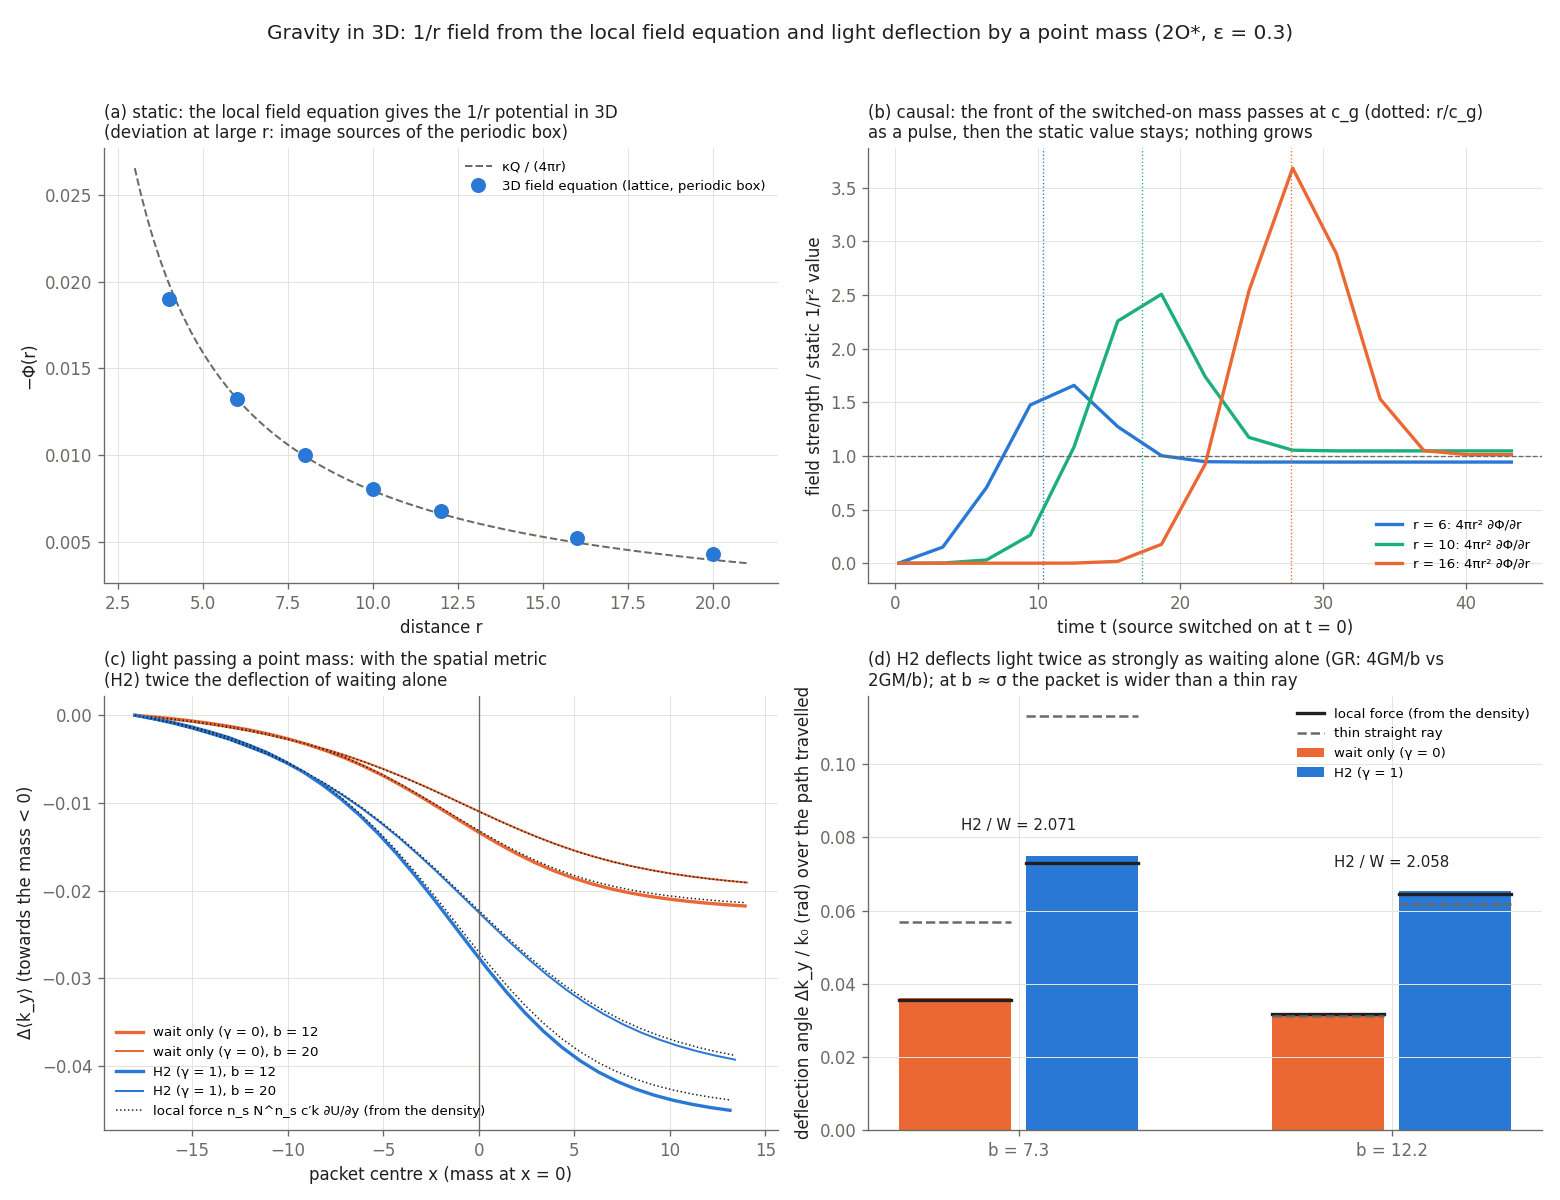
\includegraphics[width=0.92\textwidth]{phase_bit_s4_open12.png}
  \caption{Gravity in 3D: static and causal $1/r$ field, and light deflection by
  a point mass in the full $112\times88\times80$ walker; the budget rule (H2)
  deflects $2.07$ times more strongly than waiting alone (W).}
  \label{fig:3d}
\end{figure*}

\subsection{Newton's law and the perihelion}

A resting massive packet ($m=0.3$, $\sigma=5$) in the field of a point mass
follows the local force of the metric,
$-\langle\partial_x N\sqrt{m^{2}+(N^{n}\cpr k)^{2}}\rangle$, to $\le1\%$ for
$r\ge13$; the force lies $8\%$ (W) and $28\%$ (H2) above $mGM/r^{2}$ because the
packet's momentum spread ($v^{2}\approx0.18$) gravitates too.
A wave packet on a classical orbit is out of reach ($L\approx1\hbar$, spreading
much faster than one period), so the perihelion is computed from the classical
orbits ($a=1600$) of the walker's effective Hamiltonian
$H=N\sqrt{m^{2}+\cpr^{2}p^{2}/A^{2}}$:

\begin{center}
\begin{tabular}{lccc}
\toprule
variant & $(\gamma,\beta)$ & /PPN & /GR\\
\midrule
H2, $A=1/N$ & $(1,1)$ & $1.0026$ & $1.00$\\
wait only, $A=1$ & $(0,1)$ & $1.0011$ & $\nicefrac13$\\
linear lapse & $(1,\nicefrac12)$ & $1.0039$ & $\nicefrac76$\\
\bottomrule
\end{tabular}
\end{center}

\noindent
The PPN formula $(2+2\gamma-\beta)/3$ holds for all three; the budget rule with
the product law gives the full GR advance.
A classical orbit with $H\supset\bvec\cdot\pvec$ precesses its node at the
Lense--Thirring rate to $1.001$.

\subsection{What an observer inside the lattice sees}

An observer defines spheres by their own signals (radar time).
The cuboctahedral graph shells are invisible to them---no signal follows graph
distance; the weight of a point source at graph distance $\ge0.8n$
falls from $0.021$ at $n=8$ to below $10^{-3}$ for $n\ge32$.
What they can test is agreement between probes.
Over $2000$ directions the speed of the massless doublet varies by
$1.1\times10^{-4}$ at $k=0.05$ ($\propto k^{1.83}$, a $k^{3}Y_4$ term) and
depends on energy as $v=\cpr(1-\xi(ka)^{2})$, $\xi=0.42\pm0.05$.
Michelson--Morley with long-wavelength light finds nothing to order $(ka)^{2}$;
the particle's own isotropy improves as $C_4\propto\sigma^{-4}$ with packet
width.

% ─────────────────────────────────────────────────────────────────────────────
\section{The gravitational atom}
\label{sec:atom}
% ─────────────────────────────────────────────────────────────────────────────

A bound state is the sharpest test of a metric: level shifts are measured as
frequencies, to many digits.
For a light particle the ``gravitational atom'' has $L\sim\hbar$, so it is the
quantum counterpart of the perihelion problem.

\subsection{Effective Hamiltonian and $l$-splitting}

On a 1D chain of $512$ layers ($\mu=0.08$, $GM=0.6$, $60\,000$ ticks) the lattice
levels agree with the effective Hamiltonian
$H=N^{\nicefrac12}\sqrt{m^{2}+\cpr^{2}\Pi^{2}}\,N^{\nicefrac12}$,
$\Pi^{2}=N^{n/2}(-\nabla N^{n}\nabla)N^{n/2}$, to $0.2\%$ (ground) to $3\%$,
including the difference between H2 and W.
In 3D (radial, effective) the relativistic $l$-splitting is the quantum
perihelion: wait-only/H2 tends to $0.22\to0.31$ (classically $\nicefrac13$),
linear/H2 to $1.16$--$1.18$ ($\nicefrac76$), scaling as $(GM)^{4}$.

\subsection{Fine structure: the de Sitter factor $2\gamma+1$}

For a Dirac particle in $ds^{2}=-N^{2}dt^{2}+A^{2}d\mathbf{x}^{2}$,
$H=\beta mN+\tfrac{\cpr}{2}\{N/A,\boldsymbol{\alpha}\cdot\pvec\}$, the
Foldy--Wouthuysen expansion contains
\begin{equation}
  H_{\mathrm{SO}}=(2\gamma+1)\,\frac{\cpr^{2}}{4m}\,\frac1r\frac{dU}{dr}\,
  \vsig\cdot\mathbf{L},
\end{equation}
i.e.\ $\gamma+\nicefrac12$ per unit of spin (de~Sitter precession $\nicefrac32$
for $\gamma=1$, the Hehl--Ni term $\nicefrac12$ for $\gamma=0$~\cite{hehl1990}).
Hence $E(2p_{3/2})-E(2p_{1/2})$ is in the ratio $1:3:3$ for wait-only : H2 :
linear lapse, which the radial 2D Dirac reference confirms at weak coupling
($1:2.997:3.011$) and turns into $1:3.64:4.50$ at $\alpha_f=m\,GM/\cpr=0.3$.

A 3D atom does not fit into memory, but a 2D atom in a slab of the full 3D
walker does, and suffices because spin and orbital angular momentum are both
normal to the slab.
We run \texttt{Walker3D} on $340\times340\times2$ ($\mu=0.1$, $\alpha_f=0.3$,
Bohr radius $a_0=9.62$, $r_c=a_0/2$, $8000$ ticks), start from the reference
$2p$ shell times $e^{i\varphi}$ times a rest spinor with $J_z=\pm\nicefrac12$,
project exactly onto the $C_4$ sector, and extract the level by filter
diagonalisation of the autocorrelation~\cite{mandelshtam1997} (the FFT
resolution is $4$--$15$ times too coarse).
The reference includes the spin-independent Wilson-like term of the lattice
band ($r_b=-0.037$, measured from the band, not fitted):

\begin{center}
\begin{tabular}{lccc}
\toprule
rule & lattice ($10^{-4}$) & Dirac + $r_b$ & ratio\\
\midrule
wait only ($\gamma=0$) & $1.0715$ & $1.0881$ & $0.985$\\
H2 ($\gamma=\beta=1$) & $3.9928$ & $3.9621$ & $1.008$\\
linear ($\gamma=1,\beta=\nicefrac12$) & $4.9590$ & $4.9009$ & $1.012$\\
\bottomrule
\end{tabular}
\end{center}

\noindent
The walker has the gravitational spin--orbit coupling with the right size and
sign ($2p_{3/2}$ above $2p_{1/2}$), and its dependence on spatial curvature:
H2/W $=3.73$ against $3.64$.
Absolute $2p$ levels agree to $0.3$--$1.1\%$ (Fig.~\ref{fig:atom}).

\subsection{Hyperfine structure: Lense--Thirring}

A rotating central body adds
$\bvec=B_J\,\hat{\mathbf{z}}\times\rvec/(r^{2}+r_{c,b}^{2})^{3/2}$.
The walker couples through the drag hop ($\bvec\cdot\pvec=(b_\varphi/\rho)L_z$) and
the gyroscope rule ($\tfrac12\nabla\times\bvec\cdot\Jint$).
Far from the core, orbit : spin $=2:-1$ as in GR
($2GJ\cdot L/c^{2}r^{3}$ and $\Omega_{\mathrm{LT}}=-GJ/c^{2}r^{3}$ in the
equatorial plane), so the shifts are $\propto m_l-s_z/2$ and
$2p_{3/2}:2p_{1/2}=3:5$; without spin coupling $1:1$, with $g=2$, $1:3$.
The ratio measures the gyrogravitomagnetic factor.
With the core ($r_{c,b}=0.25a_0$) and strong field the Dirac reference gives
$0.560$.
Six lattice runs ($\pm J$, with and without the spin rule, $4.9$\,h each):

\begin{center}
\begin{tabular}{lccc}
\toprule
shift ($10^{-5}$) & lattice & reference & ratio\\
\midrule
$2p_{3/2}$, orbit only & $4.808$ & $4.678$ & $1.028$\\
$2p_{1/2}$, orbit only & $6.357$ & $6.187$ & $1.027$\\
$2p_{3/2}$, orbit + spin & $4.295$ & $4.151$ & $1.035$\\
$2p_{1/2}$, orbit + spin & $7.618$ & $7.407$ & $1.028$\\
spin part $2p_{3/2}$ & $-0.646$ & $-0.659$ & $0.980$\\
spin part $2p_{1/2}$ & $+1.077$ & $+1.036$ & $1.039$\\
\bottomrule
\end{tabular}
\end{center}

\noindent
The ratio $2p_{3/2}:2p_{1/2}$ is $0.5638$ on the lattice against $0.5604$
(orbit only: $0.7564$ vs $0.7560$), and even the part quadratic in $J$ agrees
to $4$--$6\%$.
The common factor $1.03$ of all orbital shifts is spin-independent; it is
either the slightly more compact lattice shell or the drag hop itself
($+1.5\%$ in the rigid-rotation test), not yet separated.

\begin{figure*}[t]
  \centering
  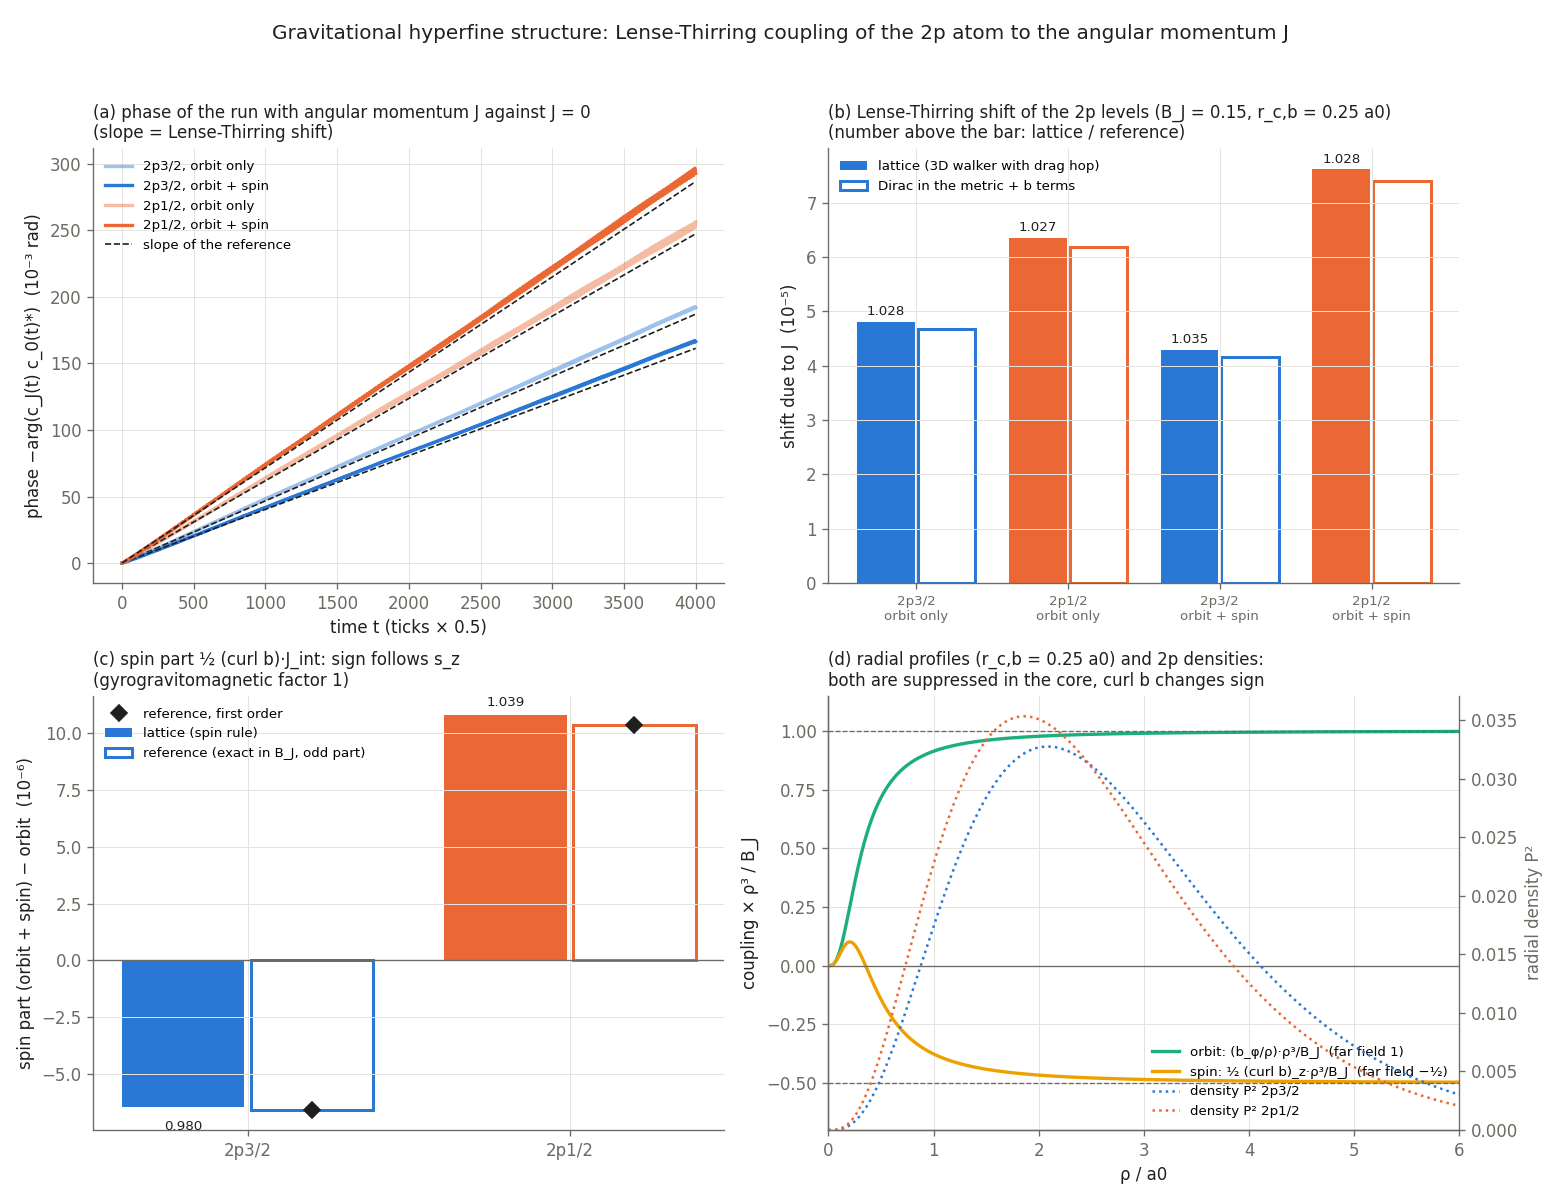
\includegraphics[width=0.92\textwidth]{phase_bit_s4_open16.png}
  \caption{Gravitational hyperfine structure.
  (a) Phase of the run with angular momentum $J$ against $J=0$; the slope is the
  Lense--Thirring shift. (b) Shifts of the $2p$ levels, lattice against the
  Dirac equation with gravitomagnetic terms. (c) Spin part: its sign follows
  $s_z$ (gyrogravitomagnetic factor~1). (d) Radial profiles of the orbital and
  spin couplings with the $2p$ densities.}
  \label{fig:atom}
\end{figure*}

% ─────────────────────────────────────────────────────────────────────────────
\section{Discussion}
\label{sec:discussion}
% ─────────────────────────────────────────────────────────────────────────────

\subsection{What follows from the rules, and what is imposed}

\emph{Derived from local rules:} spin $\nicefrac12$, Kramers and the belt-trick
sign from a finite register; the Dirac mass as reversal without spin rotation;
the lapse as the waiting fraction of a node; $\gamma=1$ from counting the nodes a
process involves; $\beta=1$ from combining loads as independent occupations;
the source $T_{00}+T_{ii}$ and proper time from the computational load; the
coefficient $C=4$ of the drag from the relativity principle; and the
quantitative agreement of all bound-state tests with the Dirac equation in the
resulting metric.

\emph{Imposed:}
(i) the field equations for $\Phi$ and $\bvec$ (Poisson or wave equation with the
measured sources)---the budget rule says how a node reacts to its load, not how
the load spreads;
(ii) the vacuum counterterm and the $\lambda(N)$ retuning;
(iii) the gyroscope rule $\tfrac12\nabla\times\bvec\cdot\Jint$, which the lattice
does not enforce (the bare spin index gives $g=-\nicefrac13$);
(iv) the equal weighting of departure and arrival nodes ($N_w=N_h$).

\subsection{Lattice signatures}

The model is not GR on a grid; it has its own predictions:
\begin{itemize}
\item \emph{Mirror instead of horizon.} Approaching $N\to0$ a photon is
blue-shifted up to the band maximum at $k=\pi/a$ and then turns back
($N=0.089$ in our run); massive particles bounce back almost to their starting
height.
\item \emph{Energy-dependent light speed} $1-0.42(ka)^{2}$ and a cubic
anisotropy $\propto(ka)^{2}$; quadratic in $a$, this is compatible with
gamma-ray-burst timing if $a$ is near the Planck length.
\item \emph{Vacuum energy.} The Floquet offset gravitates unless subtracted, and
the Dirac sea must be normal ordered---the cosmological-constant problem
appears explicitly as a lattice counterterm.
\item \emph{Background of order $\Delta t$} from the stay gate, which breaks
local Lorentz invariance at finite $k$ in loaded regions unless compensated.
\end{itemize}

\subsection{Open problems}

The decisive open question is the \emph{tensor sector}.
The model has two scalars ($N$, $A=1/N$) and a vector ($\bvec$); GR also has
transverse-traceless radiation.
Many theories reproduce $\gamma=\beta=1$ in the static weak field and fail on
gravitational waves.
Whether an oscillating load on the lattice radiates two tensor polarisations,
or whether the budget rule is a scalar--vector theory that only mimics GR in the
solar system, is the next test.
Equally important is a derivation of the gyroscope rule from a drag hop that
also rotates the $\Ot$ register, and a field equation for $\Phi$ and $\bvec$ that
follows from the node rule rather than being added to it.

% ─────────────────────────────────────────────────────────────────────────────
\section{Conclusion}
\label{sec:conclusion}
% ─────────────────────────────────────────────────────────────────────────────

A unitary walker with a finite spin register and one local node rule---every
process needs each node it involves to be free---reproduces the post-Newtonian
limit of general relativity with $\gamma=\beta=1$, full light bending in
\mbox{3\!+\!1D}, the GR perihelion advance, the Lense--Thirring dipole, and the
fine and hyperfine structure of a gravitational atom to a few percent.
Nordstr\"om, Einstein~1911 and GR appear as successive rungs: slow the clock,
slow everything, slow hops twice.
Gravity, in this model, is the bookkeeping of which nodes are busy.

% ─────────────────────────────────────────────────────────────────────────────
\begin{acknowledgments}
Numerical simulations and analysis were implemented with the assistance
of Claude Code (Anthropic, claude-opus-5-5).
\end{acknowledgments}

% ─────────────────────────────────────────────────────────────────────────────
\begin{thebibliography}{99}

\bibitem{schmiereck2026}
  T.~Schmiereck,
  ``Relativistic Quantum Mechanics from Lattice Geometry:
    Emergent Speed of Light, Mass, and Time Dilation on an Equilateral
    Triangular Lattice,''
  Zenodo (2026),
  \href{https://doi.org/10.5281/zenodo.22178585}{doi:10.5281/zenodo.22178585}.

\bibitem{schmiereck2026b}
  T.~Schmiereck,
  ``Internal Structure of the Equilateral Lattice Path Integral:
    Crystal Angular Momentum, Emergent Vector Ground State,
    and Symmetry Breaking by Confinement,''
  Zenodo (2026),
  \href{https://doi.org/10.5281/zenodo.23888331}{doi:10.5281/zenodo.23888331}.

\bibitem{einstein1911}
  A.~Einstein,
  ``\"Uber den Einflu{\ss} der Schwerkraft auf die Ausbreitung des Lichtes,''
  \emph{Ann.\ Phys.}\ \textbf{35}, 898 (1911).

\bibitem{will2014}
  C.~M.~Will,
  ``The confrontation between general relativity and experiment,''
  \emph{Living Rev.\ Relativ.}\ \textbf{17}, 4 (2014).

\bibitem{aharonov1993}
  Y.~Aharonov, L.~Davidovich, and N.~Zagury,
  ``Quantum random walks,''
  \emph{Phys.\ Rev.\ A}\ \textbf{48}, 1687 (1993).

\bibitem{strauch2006}
  F.~W.~Strauch,
  ``Relativistic quantum walks,''
  \emph{Phys.\ Rev.\ A}\ \textbf{73}, 054302 (2006).

\bibitem{hehl1990}
  F.~W.~Hehl and W.-T.~Ni,
  ``Inertial effects of a Dirac particle,''
  \emph{Phys.\ Rev.\ D}\ \textbf{42}, 2045 (1990).

\bibitem{mandelshtam1997}
  V.~A.~Mandelshtam and H.~S.~Taylor,
  ``Harmonic inversion of time signals and its applications,''
  \emph{J.\ Chem.\ Phys.}\ \textbf{107}, 6756 (1997).

\bibitem{repo}
  T.~Schmiereck, \texttt{hex\_field\_map},
  \url{https://github.com/schmiereck/hex_field_map}
  (scripts \texttt{src/phase\_bit\_*.py}, results \texttt{docs/RESULTS\_*\_de.md}).

\end{thebibliography}

\end{document}
